\documentclass{article}
\usepackage{amsmath}
\usepackage{graphicx}
\usepackage[a4paper, margin=1in]{geometry}
\usepackage{pgfplots}
\pgfplotsset{compat=1.17}
\usepackage{afterpage}
\usepackage{float}
\usepackage{hyperref}
\usepackage{subcaption}
\graphicspath{{assets/}}

\title{Producers Consumers}
\author{Epameinondas Bakoulas}
\date{May 2025}

\begin{document}

\maketitle

\section{Modifications on the Producer Consumer Problem}

The producer consumer problem is a classic synchronization problem in computer science. 
It involves two types of processes: producers, which generate data and place it into a buffer, 
and consumers, which take data from the buffer. The challenge is to ensure that the producer 
does not add data to a full buffer and the consumer does not remove data from an empty buffer.

Using the already implemented version of the producer consumer problem from Andrae Muys, we
will make some modifications to the code and add some features. On the fifo queue, we will add a
work function that will take a function pointer as an argument. It will also take a pointer to an
array of arguments. Out goal is for the consumer to insert some values into the buffer (e.g. 10 angles)
and the producer to take them out and apply a function on them (e.g. calculate the sine of the angles).

Our goal is to \textbf{measure the average waiting time} of the values in the buffer. We will work with a
a lot of different number of producers and consumers, and aim to find the optimal number of
consumers for a given number of producers.

\section{Implementation}

As said before, we will work on top of the already implemented version of the producer consumer problem 
from Andrae Muys. Inside the queue, we will add the following \texttt{workFunction}:

\begin{verbatim}
struct workFunction {
    void* (*work)(void*);
    void* arg;
    struct timeval enqueue_time;
    struct timeval dequeue_time;
};
\end{verbatim}

Where \texttt{work} is a function pointer to the function that will be executed by the consumer,
in our case the \texttt{calculate\_sine} function. \texttt{arg} is a pointer to the arguments of the function,
in our case 10 angles. \texttt{enqueue\_time} and \texttt{dequeue\_time} are the times that the work function was
enqueued and dequeued from the queue. We will use these times to calculate the average waiting time of the work function.

\section{Benchmarks}
We will work with a queue of size 10 in all of the tests, and the producers will create a total of
$ producer * 100000 $ \texttt{workFunction}s. This number is arbitrary, but we want to have a
large enough number of \texttt{workFunction}s to be able to measure the average waiting time.

The specs of the computer that we will run the tests are: CPU: Intel Core i5-11400F (6 cores, 12 threads), RAM: 16GB, OS: Linux Mint 22.

The following graphs shows the average waiting time for a different number of producers and consumers.

\begin{figure}[H]
    \centering
    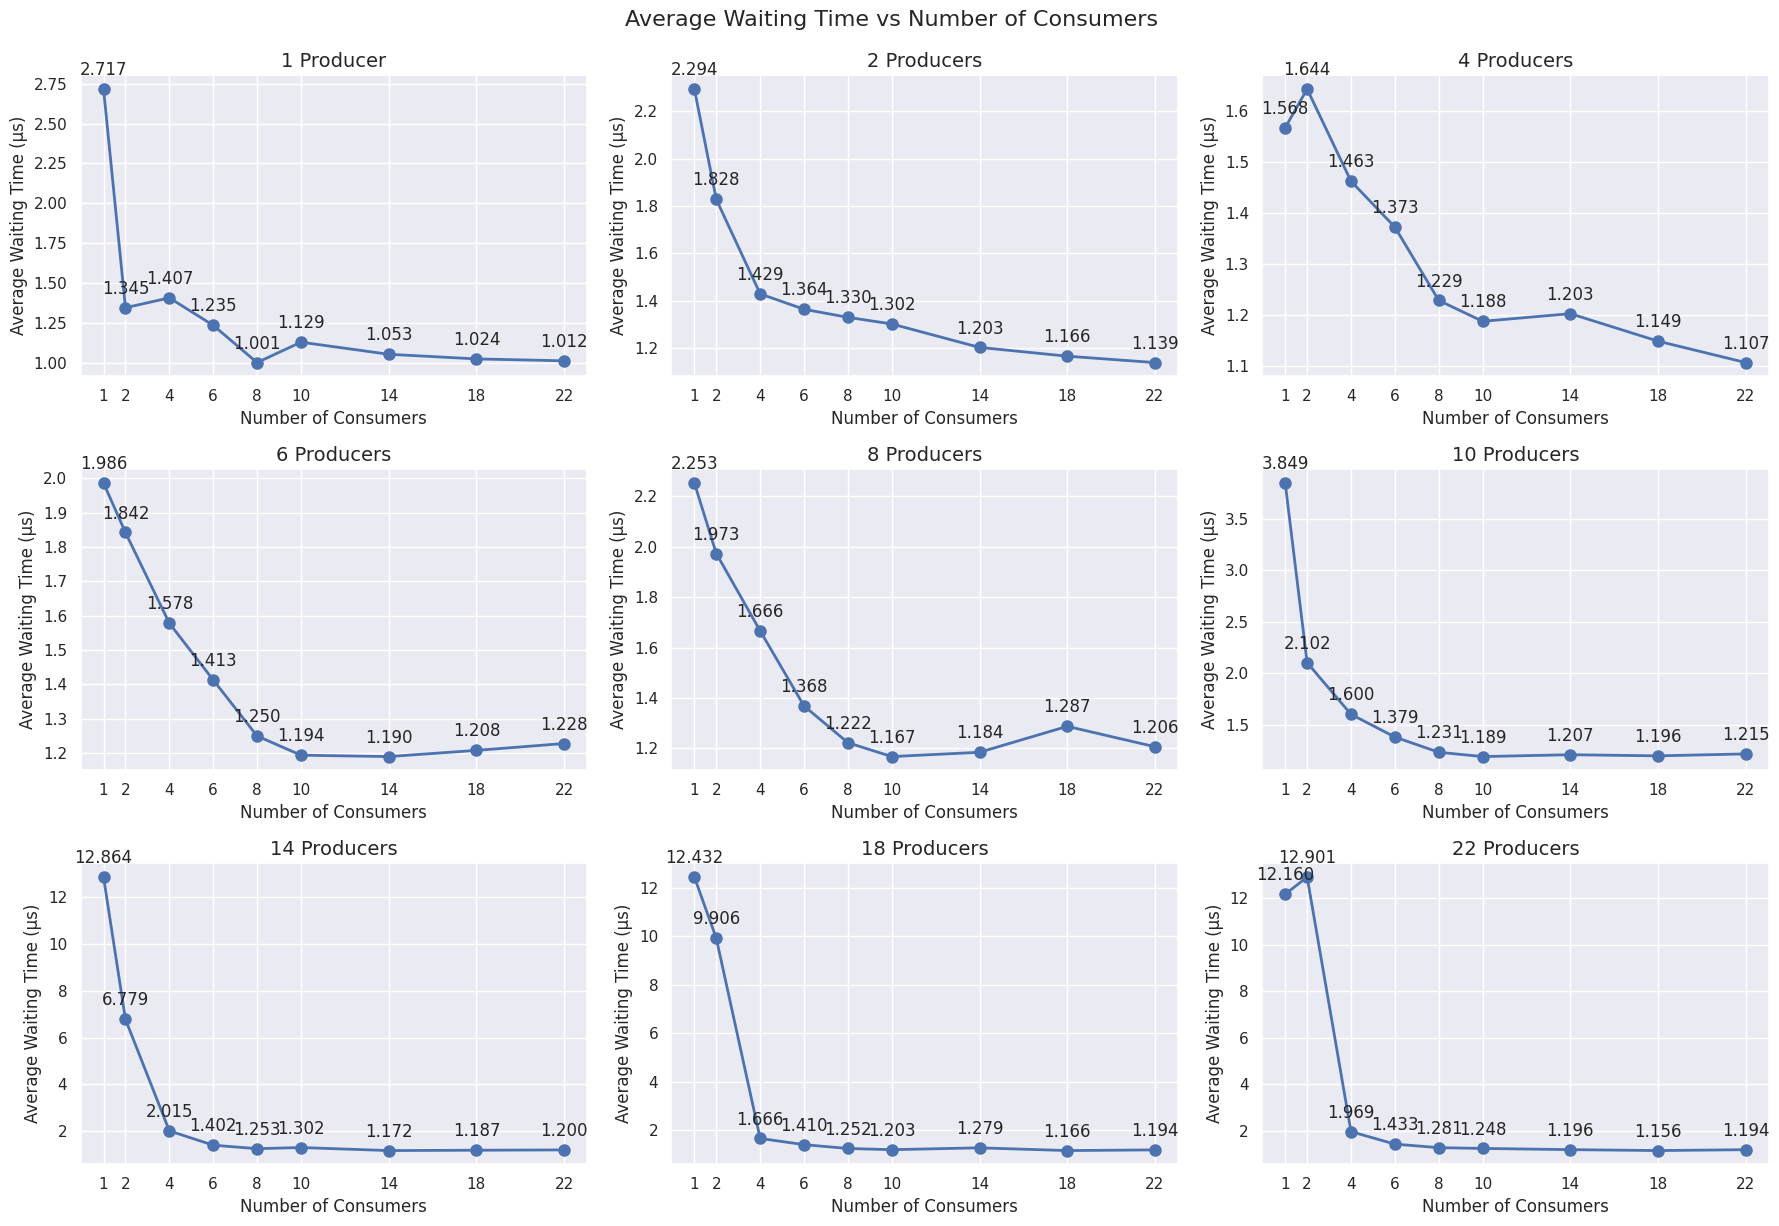
\includegraphics[width=1\textwidth]{benchmarks.png}
    \caption{Benchmarks of the average waiting time for different number of producers and consumers.}
    \label{alg:benchmarks}
\end{figure}

As we can see, having around \textbf{8-10 consumers} seems to be the optimal number for a given number of producers.
Comparatively, 1-2 consumers seems to perform relatively bad, while having over 10 consumers seems to not give us
a meaningful performance boost. All in all, having 8 and above consumers seems to be the optimal number.

\section{Conclusion}

From the benchmarks we can see that the average waiting time is not linear with the number of producers and consumers.
Increasing the consumers from a certain point does not give us a meaningful performance boost.
If we want to minimize the number of threads that we use, we can use around 8 consumers and we will be able to
achieve a relative good performance.

The source code can be found on the \href{https://github.com/NontasBak/producer-consumer}{Github repository}.


\end{document}